%; whizzy chapter -dvi
% -initex iniptex -latex platex -format platex -bibtex jbibtex -fmt fmt
% 以上 whizzytex を使用する場合の設定。

%     Tokyo Debian Meeting resources
%     Copyright (C) 2012 Junichi Uekawa
%     Copyright (C) 2012 Nobuhiro Iwamatsu

%     This program is free software; you can redistribute it and/or modify
%     it under the terms of the GNU General Public License as published by
%     the Free Software Foundation; either version 2 of the License, or
%     (at your option) any later version.

%     This program is distributed in the hope that it will be useful,
%     but WITHOUT ANY WARRANTY; without even the implied warranty of
%     MERCHANTABILITY or FITNESS FOR A PARTICULAR PURPOSE.  See the
%     GNU General Public License for more details.

%     You should have received a copy of the GNU General Public License
%     along with this program; if not, write to the Free Software
%     Foundation, Inc., 51 Franklin St, Fifth Floor, Boston, MA  02110-1301 USA

%  preview (shell-command (concat "evince " (replace-regexp-in-string "tex$" "pdf"(buffer-file-name)) "&"))
% 画像ファイルを処理するためにはebbを利用してboundingboxを作成。
%(shell-command "cd image201205; ebb *.png")

%%ここからヘッダ開始。

\documentclass[mingoth,a4paper]{jsarticle}
\usepackage{monthlyreport}

% 日付を定義する、毎月変わります。
\newcommand{\debmtgyear}{2012}
\newcommand{\debmtgmonth}{10}
\newcommand{\debmtgdate}{20}
% (+ (* (- 2012 2005) 12) 10 -1) started from zero
\newcommand{\debmtgnumber}{93}

\begin{document}

\begin{titlepage}
\thispagestyle{empty}
% タイトルページ:編集必要な部分は最初のマクロに飛ばすこと

\vspace*{-2cm}
第\debmtgnumber{}回 東京エリア Debian 勉強会資料\\
\hspace*{-2cm}

\includegraphics{image2012-natsu/dotdeb.pdf}\\
\hfill{}\debmtgyear{}年\debmtgmonth{}月\debmtgdate{}日

% ここはアップデートすること
% 全角文字にしないとフォントのサイズが合わないので注意
% TODO(uekawa): なんでそうなるのか確認
\rotatebox{10}{\fontsize{32}{32} {\gt 特集: Haskellパッケージ}}\\
\rotatebox{10}{\fontsize{32}{32} {\gt 特集: mtrack}}\\

\vspace*{-2cm}
\hfill{}
\includegraphics[height=6cm]{image200502/openlogo-nd.eps}
\end{titlepage}

% Title should be in Japanese text so that we can use it as lint for PDF shiori.
\dancersection{はじめに}{上川 純一}

\begin{multicols}{2}
 

 今月のDebian勉強会へようこそ。これからDebianの世界にあしを踏み入れると
 いう方も、すでにどっぷりとつかっているという方も、月に一回Debianについ
 て語りませんか?

 Debian勉強会の目的は下記です。

 \begin{itemize}
 \item \underline{Debian Developer} (開発者)の育成。
 \item 日本語での「\underline{開発に関する情報}」を整理してまとめ、アップデートする。
 \item \underline{場}の提供。
 \begin{itemize}
  \item 普段ばらばらな場所にいる人々が face-to-face で出会える場を提供
	する。
  \item Debian のためになることを語る場を提供する。
  \item Debianについて語る場を提供する。
 \end{itemize}
 \end{itemize}		

 Debianの勉強会ということで究極的には参加者全員がDebian Packageをがりがり
 と作るスーパーハッカーになった姿を妄想しています。情報の共有・活用を通し
 て Debianの今後の能動的な展開への土台として、「場」としての空間を提供す
 るのが目的です。

\end{multicols}

\newpage

\begin{minipage}[b]{0.2\hsize}
 \definecolor{titleback}{gray}{0.9}
 \colorbox{titleback}{\rotatebox{90}{\fontsize{80}{80} {\gt デビアン勉強会} }}
\end{minipage}
\begin{minipage}[b]{0.8\hsize}
\hrule
\vspace{2mm}
\hrule
\begin{multicols}{2}
\tableofcontents
\end{multicols}
\vspace{2mm}
\hrule
\end{minipage}

\dancersection{事前課題}{上川 純一}

今回の事前課題は以下です:
次から適当に選んで答えてください: 
\begin{enumerate}

 \item Debian での関数型プログラミング言語の利用経験とその時に感じた事柄(Lisp, Emacs Lisp, OCaml, Haskell 等) 
 \item 関数型プログラミング言語初心者に向けたお勧め書籍とそのウリの紹介, 
 \item 関数型言語で実装されている、使ってみたいソフトをあげてください
\end{enumerate}
この課題に対して提出いただいた内容は以下です。
\begin{multicols}{2}
{\small


\begin{prework}{ $B4d>>(B $B?.MN(B }

(1) erlang $B$H(BHaskell $B$r>/!9!#(B

(2) Real World Haskell$B!#%W%m%0%i%_%s%0(BErlang$B!#(B

(3) Erlang $B$N(B $B%S%k%I%7%9%F%`$G$"$k(B rebar $B$r$b$&$A$g$C$HM}2r$7$?$$!#(B


\end{prework}

\begin{prework}{ yamamoto }

(1) $B4X?t7?%W%m%0%i%_%s%08@8l$NMxMQ7P83(B $B!](B $B$J$7(B
(2) $B$*4+$a=q@R(B $B!](B $BFI$s$@$3$H!"$"$j$^$;$s(B
(3) $B;H$C$F$_$?$$%=%U%H(B $B!](B $BFC$K$J$7(B

$B$G$b!"(Bhaskell $B$O$J$s$+LLGr$=$&$@$7!"3X$s$G$_$h$&$+$J!)$H$+9M$($F$$$^$9!#(B
\end{prework}

\begin{prework}{ alice.ferrazzi }


\end{prework}

\begin{prework}{ $BNkLZ?rJ8(B }

(1)Debian $B$G$N4X?t7?%W%m%0%i%_%s%08@8l$NMxMQ7P83$H$=$N;~$K46$8$?;vJA!J(BLisp, Emacs Lisp, OCaml, Haskell $BEy!K(B
Erlang $B!&!&!&$5$o$jDxEY$G$9$,!"(BRiak$B$J$I$N<BMQ%l%Y%k$N%=%U%H%&%'%"$G;HMQ$5$l$F$$$kE@$d!"J,;64D6-$dL5Dd;_$K8@8l%l%Y%k$GBP1~$5$l$F$$$kE@$,LLGr$+$C$?$G$9!#(BRiak$B$+$i>pJs$r<h$C$?$jF~$l$?$j$9$k$@$1$J$i$PHf3SE*4JC1$KA`:n$G$-$^$7$?!#(B
Haskell $B!&!&!&$5$o$jDxEY$G$9$,!"(BHaskell$B9%$-$J?M$,B?$$$?$a3X$V$K$ONI$$8@8l$@$H46$8$^$7$?!#(B

(2) $B4X?t7?%W%m%0%i%_%s%08@8l=i?4<T$K8~$1$?$*4+$a=q@R$H$=$N%&%j$N>R2p(B
Erlang$B$O$J$+$J$+K\$,$J$+$C$?$G$9!#(BHaskell$B$O!V$9$4$$(BHaskell$B$?$N$7$/3X$\$&!*!W$,FI$_$d$9$$$h$&$K46$8$^$9$,!"$^$@M}2r$G$-$F$^$;$s!#(B

(3) $B4X?t7?8@8l$G<BAu$5$l$F$$$k!";H$C$F$_$?$$%=%U%H$r$"$2$F$/$@$5$$(B
Riak
xmonad

\end{prework}

\begin{prework}{ $B5HLn(B(yy\_y\_ja\_jp) }

(1) $B:G6a(BHaskell$B$r?($C$F$$$^$9!%(Bcabal-debian$B$r$b$&>/$7CN$j$?$$$G$9!%(B
\end{prework}

\begin{prework}{ $B%-%?%O%i(B }

(1) Haskell $BF~Lg=q$N%5%s%W%k$rF0$+$7$?DxEY!"(B
    apt-get$B$G4JC1$KF3F~$G$-$F46F0$7$?$h$&$J5-21$,!&!&!&!#(B
(2) Haskell$B$NF~Lg=q$r(B2$B:}$[$IFI$_$^$7$?$,!"6&$K(Bmonad$B$G(B
    $B:C@^$7$?!":G6a$NK\$OFI$s$G$$$J$$!#(B
(3) $BFC$K$J$7!#(B

\end{prework}

\begin{prework}{ dictoss($B?yK\!!E5=<(B) }

(1) emacs.el$B$r=q$/$/$i$$$G$J$s$H$J$/;H$C$F$$$k46$8$G$9!#%7%s%0%k%/%)!<%F!<%7%g%s$OJD$8$J$/$F$$$$>l9g$,$"$k$N$G$=$l$K8MOG$&$3$H$,$"$j$^$9!#(B
\end{prework}

\begin{prework}{ $BLn<s(B }

elisp$B$G$A$g$C$H(Bmajor mode$B$H(Bshinbum module$B$r=q$$$F$_$?$3$H$,$"$k$0$i$$$G$9!#(B
$B4X?t7?%W%m%0%i%_%s%0$H$$$&%l%Y%k$K;j$j$^$;$s$G$7$?!#(B

\end{prework}

\begin{prework}{ @Lost\_dog\_ }

 (1) Haskell:$B7?0BA4$N$"$j$,$?$_$,J,$+$C$?(B
 (2) $B!X$9$4$$(BHaskell$B$?$N$7$/3X$\$&(B!$B!Y$O4X?t7?$NJ70O5$$rPmbW$G$-$k!#K\5$$GJY6/$9$k$J$i!"$b$C$H2&F;$N%F%-%9%H$rA*$s$@$[$&$,$h$$$+$b!#(B
 (3) yi-editor
\end{prework}

\begin{prework}{ $BF|HfLn(B $B7<(B }

(1) Haskell, OCaml $B$H$b$K(B Debian $B$K$OB??t$N%Q%C%1!<%8$,$"$C$F$9$P$i$7$$$G$9!#(B

(2)
\begin{itemize}
\item {\bf $B%W%m%0%i%_%s%0(BHaskell\\ - Graham Hutton ($BCx(B), $B;3K\(B $BOBI'(B ($BK]Lu(B)]}\\
$B:G=i$KFI$`$J$i$3$l$G$9!#4X?t%W%m%0%i%_%s%0$N%H%T%C%/$rJ?0W$K2r@b$7$J$i$,(BHaskell$B$r;n$7$F$$$-$^$9!#(B
\item {\bf $B$9$4$$(BHaskell$B$?$N$7$/3X$\$&(B!\\ - Miran Lipovaa ($BCx(B), $BEDCf(B $B1Q9T(B ($BK]Lu(B), $BB<<g(B $B?r9T(B ($BK]Lu(B)}\\
$B!V%W%m%0%i%_%s%0(BHaskell$B!W$N<!$O$3$l$@$H;W$$$^$9!#$h$jJ#;($J7?$N5!G=$r$b4^$a$F(BHaskell$B$N2r@b$,?J$s$G$$$-$^$9!#(B
\item {\bf Real World Haskell $B<B@o$G3X$V4X?t7?8@8l%W%m%0%i%_%s%0(B\\
 - Bryan O'Sullivan ($BCx(B), John Goerzen ($BCx(B), Don Stewart ($BCx(B), $B;32<(B $B?-IW(B ($BK]Lu(B), $B0KEl(B $B>!Mx(B ($BK]Lu(B), $B3t<02q<R%?%$%`%$%s%?!<%a%G%#%"(B ($BK]Lu(B)}\\
$B<B:]$K(BHaskell$B$r8=>l$GMxMQ$7$F$k?M$?$A$,=q$$$?K\$H$7$F$N2ACM$,$"$kK\$G$9!#(B
Haskell$B$K$b$$$m$$$m$J%i%$%V%i%j$,$"$j!"$=$NMxMQNc$H$7$F;29M$K$J$k$H;W$$$^$9!#(B
$B>/$78E$$$N$,LdBjE@$G$9!#(B
\end{itemize}

(3) OCaml$B$G:n$i$l$F$$$kDjM}>ZL@4o(BCoq$B$r$&$^$/;H$($k$h$&$K$J$j$?$$$G$9!#$"$H(BHaskell$B$G$$$m$$$m:n$kB&$K$^$o$j$?$$!#(B

\end{prework}

}
\end{multicols}

\dancersection{最近のDebian関連のミーティング報告}{上川 純一}
\subsection{東京エリアDebian勉強会91回目報告}

% (query-replace-regexp "<.*?>" "")
% (query-replace-regexp "^[	 ]\+" "")

第91回東京エリアDebian勉強会でした。
参加者は
中尾さん、山田泰志さん、やまねひできさん、やまもとひろゆきさん、北原さん、日比野さん、吉田@板橋さん、杉本さん、野島さん、岩松さん、alice ferazzi さん、上川でした。

岩松さんがDebconfの紹介をしました。あつい。日本で開催するならどうしようかという話題でしばし盛り上がりました。
AARM64の話題とか、ClangでDebianをコンパイルしてみるプロジェクトについて語ってました。

野島さんがDebianにおいての共有ライブラリについて紹介しました。
シンボルベースのバージョンをつかってshlibsファイルに相当するものを作成する仕組みについて説明しました。
それで本当に良いのか、いい感じに議論が紛糾。	    

野島さんが簡単にできそうなDebian貢献について紹介しました。
翻訳とか、Debianartプロジェクトとか、適切なライセンスであるかのレビューだとか。

上川がC++11をDebianで使う現状について語りました。
なんでC++やねんというリアクションもいい感じでした。
実装面では、Debian experimentalに入ってきた libc++ がこれからどうなるのか楽しみです。

その後近所の居酒屋に場所を移してDebianの19歳誕生日を祝いました。


\dancersection{Debian Trivia Quiz}{岩松 信洋}

ところで、みなさん Debian 関連の話題においついていますか?Debian関連の話
題はメーリングリストをよんでいると追跡できます。ただよんでいるだけではは
りあいがないので、理解度のテストをします。特に一人だけでは意味がわからな
いところもあるかも知れません。みんなで一緒に読んでみましょう。

今回の出題範囲は\url{debian-devel-announce@lists.debian.org} や \url{debian-devel@lists.debian.org}に投稿された
内容とDebian Project Newsからです。

\begin{multicols}{2}
%; whizzy-master ../debianmeetingresume201210.tex
% 以上の設定をしているため、このファイルで M-x whizzytex すると、whizzytexが利用できます。
%

\santaku
{9/29 に行われた Debian 6.0 のアップデートは何回目でしょうか。}
{5}
{6}
{7}
{B}
{6.0.6 です。}

\santaku
{DMUA フィールドがなくなり、Debian Maintainerのアップロードが変更されます。今後、アップロードの際にどのように作業する必要があるか?}
{FTP masterに電話}
{スポンサーに dak の処理を依頼する}
{専用アップローダにアップロード}
{B}
{}

\santaku
{IRC 経由でVCS リポジトリを監視するサービスで終了したものは?}
{ICPO}
{NPA}
{CIA}
{C}
{KGBに移行。ICPA:  International Criminal Police Organization, NAP:National Police Agency, CIA: Central Intelligence Agency}

\santaku
{Debian Policy メンテナに新しく入ったのは誰か?}
{Kei Hibino}
{Colin Watson}
{Charles Plessy}
{C}
{Andrew McMillan, Colin Watson, Manoj Srivastava が抜けた}

\santaku
{Checksums-SHA1,SHA256 の取り扱いが変更になったが、どう変更されたか?}
{今まで無視されていました。ごめんね。}
{オプションだったので、必須としました。}
{これらは廃止し、SHA-512のみにします。}
{B}
{Bug\#690293}

\end{multicols}

%-------------------------------------------------------------------------------
\dancersection{Haskell周辺のDebian packaging}{日比野}
%-------------------------------------------------------------------------------
\index{haskell}

$B$3$N5-;v$G$O!"(B
$B%W%m%0%i%_%s%08@8l(BHaskell$B$N%Q%C%1!<%8$H!"(B
$B$=$N%Q%C%1!<%8$,$I$N$h$&$K0MB84X782r7h$5$l$F(BDebian$B2=$5$l$F$$$k$N$+$K$D$$$F>R2p$7$^$9!#(B

%% -Haskell $B$N%Q%C%1!<%8$*$h$S0MB84X78$N;EAH$_$G$"$k(B Cabal, Hackage,

\subsection{Hackage}

http://hackage.haskell.org/
$B$O(BHaskell$B$G=q$+$l$?%i%$%V%i%j$d%D!<%k$N%Q%C%1!<%8G[I[%5%$%H$G!"(B
Perl$B$G$N(BCPAN{\footnote{http://www.cpan.org/}}$B$N$h$&$J$b$N$G$9!#(B
$B$3$3$GG[I[$5$l$F$$$k(BHaskell$B$N%Q%C%1!<%872$O(BHackageDB$B$H8F$P$l!"(B
$B$=$l$>$l$N%Q%C%1!<%8$O$7$P$7$P(BHackage$B$H8F$P$l$^$9!#(B
$B<!$N$h$&$J(BURL$B$G$=$l$>$l$N(BHackage$B$N>pJs$r;2>H$G$-$^$9!#(B

\begin{commandline}
http://hackage.haskell.org/package/<hackage$B$NL>A0(B>
\end{commandline}

$B3F(BHackage$B$N%=!<%9%3!<%I$N(Btarball$B$K$O!"(B
$B%P!<%8%g%s>pJs$d%i%$%V%i%j!"%S%k%I%D!<%k$N0MB84X78>pJs$,4^$^$l$F$$$^$9!#(B

{\bf language-objc$B%Q%C%1!<%8$NNc(B:}

\begin{commandline}
Name:          language-objc
Version:       0.4.2.5
...
Library
...
    Build-Depends: base       >= 3 && < 5,
                   filepath   >= 1.1 && < 1.4,
                   process    == 1.1.*,
                   directory  >= 1.1 && < 1.3,
                   array      == 0.4.*,
                   containers >= 0.4     && < 0.6,
                   newtype    == 0.2.*,
                   pretty     == 1.1.*
...
    Build-Tools:    happy, alex
\end{commandline}

\subsection{Cabal\protect\footnote{http://hackage.haskell.org/package/Cabal} $B%i%$%V%i%j$H(B
cabal-install\protect\footnote{http://hackage.haskell.org/package/cabal-install}}

Cabal$B$O0MB84X78$K$7$?$,$C$F%Q%C%1!<%8$r(BHackage$B$N%5%$%H$+$i<h$C$F$-$?$j!"(B
$B%Q%C%1!<%8$N%=!<%9%D%j!<$H<j85$N4D6-$+$i%Q%C%1!<%8$r(Bbuild$B$7$?$j$9$k%i%$%V%i%j$G$9!#(B

cabal-install$B$O(BCabal$B%i%$%V%i%j$r%3%^%s%I%i%$%s$+$i8F$S=P$9$?$a$N%D!<%k$G$9!#(B
Hackage$B$NL>A0$O(Bcabal-install$B$G$9$,!"%3%^%s%I$NL>A0$O(B cabal$B$G$9!#4JC1$JMxMQJ}K!$ONc$($P0J2<$N$h$&$J46$8$K$J$j$^$9!#(B

\begin{commandline}
% cabal unpack language-objc ## hackage.haskell.org$B$+$i$N<hF@$HE83+(B
% cd language-objc-0.4.2.5
% cabal configure            ## $B0MB84X78$N8!::(B
% cabal build                ## $B%3%s%Q%$%k(B
% cabal copy                 ## $B%$%s%9%H!<%k(B
% cabal register             ## $B%$%s%9%H!<%k4IM}>pJs$r=hM}7O$KEPO?(B
\end{commandline}

$B$"$k$$$O(B

\begin{commandline}
% cabal install language-objc  ## $B:F5"E*$K%$%s%9%H!<%k$rA4$F<B9T(B
\end{commandline}

Cabal$B%i%$%V%i%j(B, cabal-install $B$N$I$A$i$b(B Haskell $B$G=q$+$l$F$$$F(B HackageDB $B$KCV$+$l$F$$$^$9!#(B
$B8=:_$N;v<B>eI8=`$N(BHaskell$B=hM}7O$O(BGlasgow Haskell Compiler(GHC)$B$G$9$,!"(B
Cabal$B%i%$%V%i%j$O(BGHC$B$N%=!<%9%D%j!<$K4^$^$l$k7A$GG[I[$5$l$F$$$^$9!#(B
$BDL>o$N3+H/4D6-$GMxMQ$5$l$k$N$O$3$N4^$^$l$F$$$k(BCabal$B%i%$%V%i%j$G$9!#(B

%% -$B$=$N>pJs$rMxMQ$7$F(B Debian $B%Q%C%1!<%8$r:n$k(B cabal-debian $B%3%^%s%I$*$h$S(B debian $B%i%$%V%i%j(B,

\subsection{debian\protect\footnote{http://hackage.haskell.org/package/debian} $B%i%$%V%i%j$H(B
cabal-debian\protect\footnote{http://hackage.haskell.org/package/cabal-debian} }

debian$B$O(BDebian$B%=!<%9%Q%C%1!<%8$N>pJs$r%O%s%I%j%s%0$9$k$?$a$N%i%$%V%i%j$G$9!#(B
$B$3$N%i%$%V%i%j$r;H$C$F:n$i$l$F$$$k(Bcabal-debian$B$H$$$&%D!<%k$G!"(B
$B<!$N$h$&$K(BHackage$B$N%=!<%9$r(BDebian$B$N%=!<%9%Q%C%1!<%8$KJQ49$9$k$3$H$,$G$-$^$9!#(B

\begin{commandline}
% cabal unpack language-objc
% cd language-objc-0.4.2.5
% cabal-debian --debianize
\end{commandline}

$B<!$N$h$&$K$&$^$/0MB84X78$N>pJs$,JQ49$5$l$^$9!#(B

\begin{commandline}
% cat debian/control
Source: haskell-language-objc
Priority: extra
Section: haskell
...
Build-Depends: debhelper (>= 7.0),
               haskell-devscripts (>= 0.8),
               cdbs,
               ghc,
               ghc-prof,
               libghc-newtype-dev (>= 0.2) | libghc-newtype-dev (<< 0.3),
               libghc-newtype-prof (>= 0.2) | libghc-newtype-prof (<< 0.3),
               libghc-syb-dev (>= 0.3) | libghc-syb-dev (<< 0.4),
               libghc-syb-prof (>= 0.3) | libghc-syb-prof (<< 0.4),
               happy,
               alex
Build-Depends-Indep: ghc-doc,
                     libghc-newtype-doc (>= 0.2) | libghc-newtype-doc (<< 0.3),
                     libghc-syb-doc (>= 0.3) | libghc-syb-doc (<< 0.4)
...
\end{commandline}

$B%i%$%V%i%j$N%Q%C%1!<%8$@$H!"$=$N$^$^MxMQ$G$-$kDxEY$N$b$N$,<+F0E*$K@8@.$5$l$^$9!#(B
$B<B9T%U%!%$%k$,$"$k$b$N$K$D$$$F$O(Brules$B$K%$%s%9%H!<%k@h$r=q$/I,MW$,$"$j$^$9!#(B

$B8=:_$N(BDebian$B$G$O(B libghc-<hackage$B$NL>A0(B>-{dev,prof,doc} $B$H$$$&L>A0$G(B Debian$B%Q%C%1!<%8$,:n$i$l$^$9!#(B
libghc-*-dev$B$O3+H/MQ%i%$%V%i%j!"(Blibghc-*-prof$B$O%W%m%U%!%$%k>pJs<hF@MQ$N%i%$%V%i%j!"(Blibghc-*-doc$B$O%i%$%V%i%j%I%-%e%a%s%H$G$9!#(B

Haskell$B$N>l9g$O(B haddock $B$H$$$&%D!<%k$G%=!<%9%3!<%IFb$NFCDj$N7A<0$N%3%a%s%H$,%I%-%e%a%s%H$KJQ49$5$l$^$9!#(B
libghc-*-doc$B$O$3$3$+$i:n$i$l$^$9!#(B

%% -Debhelper $B$H$NO"7H$N$?$a$N%9%/%j%W%H$G$"$k(B haskell-devscripts

\subsection{haskell-devscripts}

cabal-debian $B$G:n$i$l$?(BDebian$B$N%=!<%9%Q%C%1!<%8$O(B
haskell-devscripts $B$K4^$^$l$F$$$k(Bcdbs$BMQ$N(BMakefile (hlibrary.mk)$B$r(B
$BMxMQ$9$k$h$&$K9=@.$5$l$F$$$^$9!#(B

\begin{commandline}
% cat debian/rules
#!/usr/bin/make -f
include /usr/share/cdbs/1/rules/debhelper.mk
include /usr/share/cdbs/1/class/hlibrary.mk

# How to install an extra file into the documentation package
#binary-fixup/libghc-language-objc-doc::
#	echo "Some informative text" > debian/libghc-language-objc-doc/usr/share/doc/libghc-language-objc-doc/AnExtraDocFile
\end{commandline}

dh\_haskell\_* $B$N%3%^%s%I72$O(Bhlibrary.mk $B$+$iMxMQ$5$l$F$$$^$9!#(B
$B3F%3%^%s%I$O4pK\E*$K$O(BGHC$B$N%$%s%9%H!<%k>pJs4IM}MQ$N%U%!%$%k(B(debian/*/var/lib/ghc/package.conf.d/*.conf)$B$rMxMQ$7$D$D!"(B*.substvars$B$r=PNO$7$^$9!#(B

\begin{description}
\item[dh\_haskell\_depends] Haskell$B$N%i%$%V%i%j$N0MB84X78$r(BDebian$B$N0MB84X78$KJQ49$7$^$9!#(B
\item[dh\_haskell\_extra\_depends] $B%G!<%?$N%Q%C%1!<%8$d<B9T%W%m%0%i%`$N%Q%C%1!<%8$H$$$C$?!"(B
$B%i%$%V%i%j$N0MB84X78$G$O2r7h$G$-$J$$0MB84X78$r(BDebian$B$N0MB84X78$KJQ49$7$^$9!#(B
\item[dh\_haskell\_provides] Haskell$B$N%i%$%V%i%j$N(BDebian$B2>A[%Q%C%1!<%8$b4^$a$?Ds6!>pJs$r7W;;$7$^$9!#(B
\item[dh\_haskell\_shlibdeps] Haskell$B$N%i%$%V%i%j$,0MB8$7$F$$$k(B
$B%i%$%V%i%j%"!<%+%$%V(B(*.a)$B$rDs6!$7$F$$$k%Q%C%1!<%8$r7W;;$7(BDebian$B$N0MB84X78$H$7$F=PNO$7$^$9!#(B
shlibdeps$B$J$N$K%i%$%V%i%j%"!<%+%$%V(B(*.a)$B$N$_$J$N$O!"(B
$B8=>u$N(BDebian$B$N(BGHC$B4D6-$@$H!"%i%$%V%i%j%Q%C%1!<%8$r6&M-%i%$%V%i%j$K$O%3%s%Q%$%k$7$F$$$J$$$+$i$G$9!#(B
\end{description}

\subsection{$B$*$o$j$K(B}

HackageDB$B$N0MB84X784IM}$H(BDebian$B%Q%C%1!<%8$N4X78$K$D$$$F=q$$$F$_$^$7$?!#(B
$B4XO"$N%D!<%k$b$h$/$G$-$F$$$k$N$G!"(BDebian$B2=$b4JC1$=$&$K8+$($?$N$G$O$J$$$G$7$g$&$+!#(B
$B$3$N5!2q$K5$$K$J$k(BHackage$B$r(BDebian$B2=$7$F$_$F$O$I$&$G$7$g$&$+!#(B


%-------------------------------------------------------------------------------
\dancersection{レゴでなめこ収穫機を作ってみた}{本庄 弘典}
%-------------------------------------------------------------------------------
\index{lego}
\index{れごまいんどすとーむ@レゴマインドストーム}

\subsection{はじめに}

PC上で動作させたpythonスクリプトからレゴ マインドストームを操作し、
iPhoneやAndroidで人気のアプリ『なめこ栽培キット』の収穫機を作りました。
\index{なめこさいばいきっと@なめこ栽培キット}

\begin{figure}[ht]
  \begin{center}
    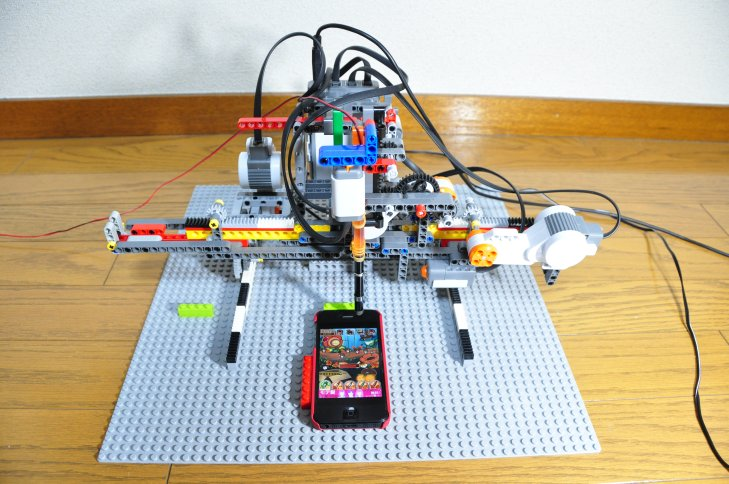
\includegraphics[width=0.7\hsize]{image201210/nxt-python_namekorobo2.jpg}
  \end{center}
  \caption{なめこロボ}
  \label{fig:namekorobo2}
\end{figure}

\subsection{『なめこ栽培キット』とは}

原木になめこの餌を注入し、
生えてきたなめこを指でなぞって収穫するiPhoneおよびAndroidのゲームです。
株式会社ビーワークスからリリースされています。

\begin{itemize}
\item 正式名称は『おさわり探偵なめこ栽培キット』。
\item iPhone版での最新作は『おさわり探偵なめこ栽培キットDeluxe』。
\item たまにレアなめこが生える。
\end{itemize}

\subsection{レゴ マインドストームの紹介}

株式会社レゴが販売している教育用ロボットで、
次のような特徴を持っています。

\begin{itemize}
\item レゴブロックを使って組み立てられる
\item レゴ テクニックシリーズのパーツを使用する
\item モーターや各種センサーを制御できる
\item ARM7のコンピュータユニットから制御する
\item ETロボコンで使われている
\end{itemize}

\subsubsection{レゴ マインドストームの購入方法}
ETロボコンの委員をやっている先生に購入方法を伺ったところ、
「(株)アフレルから買ってください」と言われました。

\begin{itemize}
\item 教育用レゴ マインドストーム 正規代理店(株)アフレル
\item \url{http://www.afrel.co.jp/}
\item 現在価格 39,900円
\end{itemize}

こちらではETロボコン用のセット販売などを行っているようですが、
特にETロボコンにこだわらない場合、
Amazon.co.jpから現在価格34,000円で購入できます。

また一部のパーツは個別に購入することが可能です。
筆者は次のお店を利用しました。

\begin{itemize}
\item ホビーショップ デジラ \url{http://www.dgla.jp/shop/}
\item LEGOパーツ専門店 ハック フィン \url{http://huckfinn-lego.com/}
\item レゴ パーツ販売ショップ「ブリッカーズ」 \url{http://www.brickers.jp/}
\end{itemize}

マインドストームにはいくつか種類がありますが、
最新のものは『レゴ マインドストーム NXT 2.0』で、
筆者もこちらを購入しました。

\subsection{nxt-python}
今回の目的はなめこ栽培キットの自動収穫機であるため、
マインドストームを自立動作させる必要がありません。
nxt-pythonはPCとマインドストーム NXTをUSBやBluetoothで接続し、
PC側で実行したスクリプトに従ってマインドストームをコントロールするためのpythonモジュールです。

nxt-pythonは次の場所で公開されています。
\begin{itemize}
\item \url{http://code.google.com/p/nxt-python/}
\end{itemize}

Debian sidにはpython-nxtというパッケージがあり、
こちらを導入することでnxt-pythonが利用できます。

\begin{commandline}
$ sudo apt-get install python-nxt
\end{commandline}
%$

\subsubsection{サンプルコード}
次のコードはポートBに接続されたモーターをパワー100、
360度回転させるサンプルコードです。

\begin{commandline}
#!/usr/bin/python

import nxt.locator
from nxt.motor import *

b = nxt.locator.find_one_brick()
m_left = Motor(b, PORT_B)
m_left.turn(100, 360)
\end{commandline}

なおドキュメントは見つからなかったため、
ソースコードを読みながら使い方を調べました。

\subsubsection{BaseMotor::turn(power, tacho\_units)}

turn()はpowerにパワーを、tacho\_unitsに角度を指定してモーターを回すメソッドです。
\begin{itemize}
\item 回りきるまで制御は帰ってこない。
\item デフォルトでは回りきったところでブレーキをかける。
\item 途中でモーターが回転しなくなると例外を飛ばす。
\item powerは-100 $\sim$ 100を指定可能。
\item powerに負の値を指定すると回転が逆になる。
\item powerに-10 $\sim$ 10くらいの値を指定しても力が弱くてモーターは回らない。
\end{itemize}

\subsubsection{Motor::weak\_turn(power, tacho\_units)}
turn()は無理矢理モーターを手で止めると怪我をするくらい強く回しますが、
weak\_turn()はモーターを弱々しく回します。

\begin{itemize}
\item 手で止めると簡単にモーターは止まる。
\item このとき例外は飛ばさない。
\item 手で軽く回すと再び回り始める。
\item tacho\_units分回ると制御が帰る。
\item 使いどころが分からない。
\end{itemize}

\subsubsection{Motor::run(power=100)}

run()は指定されたパワーでモーターを回しつづけます。
run()を実行したのち、
制御はすぐに戻ってきます。
制御が戻ってきてもモーターは回りつづけます。

\subsubsection{Motor::brake(), Motor::idle()}
brake()およびidle()はモーターを止めるメソッドです。
brake()はモーターを止めて動かないようブレーキをかけますが、
idle()は惰性で回りつづけ、
緩やかに止まります。

\subsubsection{Motor::get\_tacho()}
モーターは何度回ったかをカウントしており、
get\_tacho()メソッドでこのカウンタを取得できます。
get\_tacho()は次のの三つの値を返します。
\begin{itemize}
\item .tacho\_count
\item .block\_tacho\_count
\item .rotation\_count
\end{itemize}

\subsubsection{Motor::reset\_position(relative)}
relativeにTrueを渡すと.block\_tacho\_countを、
Falseを渡すと.rotation\_countをリセットします。

\subsubsection{Touch::is\_pressed()}
タッチセンサーが押されていればTrueを、
それ以外はFalseを返します。

\subsubsection{その他}
turn()メソッドはデフォルトの動作でブレーキをかけてくれるのですが、
指定した数値どおりに動いてはくれません。
しかしtachoは正確な値に見えるので、
これを頼りに位置指定を行う関数を定義して利用しました。

\begin{commandline}
def absturn(m, p):
    d = 1
    c = m.get_tacho().rotation_count
    q = p - c
    if q &lt; 0:
        d = -1
        q = abs(q)
    m.turn(30*d, q)
\end{commandline}
% これ、HTMLエスケープっぽいけど本当に&lt;であってるの? --uekawa

\subsection{作成されたもの}

実際に動かしているコードをgistで公開しました。
\begin{itemize}
\item \url{https://gist.github.com/3897500}
\end{itemize}

動画はYouTubeで見られます。
\begin{itemize}
\item \url{http://www.youtube.com/watch?v=uIEyWBs68c8}
\item 「レゴ なめこ」で検索すると上の方に出てきます。
\end{itemize}

\subsection{最後に}
機械制御はなかなか思ったとおりに動いてくれないことが多く、
モーターが正確な位置に動いてくれないなどの苦労に見舞われましたが、
なんとか軽減することができました。

これを機会に皆さんもレゴ マインドストーム NXTの世界を覗いてみてはいかがでしょうか。

%-------------------------------------------------------------------------------
\dancersection{xserver-xorg-input-mtrack}{岩松}
%-------------------------------------------------------------------------------
\index{xserver-xorg-input-mtrack}
\index{MacBook Pro touch pad}

Apple社のMacbook Pro の タッチパッドは 2011年(2010年?) 以降からマルチタッチに対応
したトラックパッドを使っています。以前のトラッパッドでもマルチタッチができましたが、
一部の機能しか使うことができないようです(pre-multitouchと呼ばれるようです)。
pre-multitouchでは xserver-xorg-input-synaptics ドライバで動作していたのですが、
最新のMacbook pro / air / Magic Trackpad では動作しません。これらの環境でマルチタッチを
使うためには xserver-xorg-input-mtrack / multitouch といった他のドライバを利用する必要
があります。
今回、これらの情報をまとめました。

\subsection{synaptics と mtrack}
今まで使われてきた synaptics では、
プロトコルA(図\ref{fig:protocolA})が主体です。
これはタッチIDを持っていないため、トラッキングコンタクトを
管理できません。
%ステートレス
%ステートフル

mtrack では、タッチIDをサポートしたプロトコル「プロトコルB(図\ref{fig:protocolA})」を
使います。これによりより細かいタッチパッドの制御ができるようになっています。
また、「プロトコルB」をLinuxカーネルから受信し、それをXドライバにわかりやすい
(人間にとってわかりやすい)形にデータを形成するライブラリ mtdev を
使います。

\begin{figure}[h]
\begin{center}
\includegraphics[width=0.3\hsize]{image201210/mtrack.eps}
\end{center}
\caption{関係図}
\label{fig:mtrack-relation}
\end{figure}

\begin{figure}[h]
\begin{commandline}
ABS_MT_POSITION_X x[0]
ABS_MT_POSITION_Y y[0]
SYN_MT_REPORT
ABS_MT_POSITION_X x[1]
ABS_MT_POSITION_Y y[1]
SYN_MT_REPORT
SYN_REPORT
\end{commandline}

\caption{プロトコルA}
\label{fig:protocolA}
\end{figure}

\begin{figure}[h]
\begin{commandline}
ABS_MT_SLOT 0
ABS_MT_TRACKING_ID 45
ABS_MT_POSITION_X x[0]
ABS_MT_POSITION_Y y[0]
ABS_MT_SLOT 1
ABS_MT_TRACKING_ID 46
ABS_MT_POSITION_X x[1]
ABS_MT_POSITION_Y y[1]
SYN_REPORT
\end{commandline}
\caption{プロトコルB}
\label{fig:protocolB}
\end{figure}

\subsection{multitouch と mtrack}

現在、Macbook Pro / Air 用のタッチパッドをサポートしているドライバは
multitouch とmtrack の2つがあります。multitouch が先に作られましたが、
基本的な設定しかできないシンプルな設定だったため、
mtrack という multitouch からフォークした 
ドライバが作成されました。
こちらはタッチの圧力やジェスチャーのサポートが行われているため、
使っているユーザが多いようです。

\subsection{Debian で使う}
Debian では既にパッケージ化されており、APT でインストールできます。

\begin{commandline}
$ sudo apt-get install xserver-xorg-input-mtrack
\end{commandline}
%$

インストールされると、図\ref{fig:mtrack-default}の内容の
xorg 設定ファイルが /usr/share/X11/xorg.conf.d/以下にインストール
され、xorg.conf に記述しなくても動作するようになります。

\begin{figure}[h]
\begin{commandline}
Section "InputClass"
    MatchIsTouchpad "true"
    Identifier "Multitouch Touchpad"
    Driver "mtrack"
EndSection
\end{commandline} 
\caption{mtrackのデフォルト設定}
\label{fig:mtrack-default}
\end{figure}

インストールした段階では、デフォルトの設定で動作します。
以下によく使われる設定項目を表\ref{fig:mtrack-config}示します。

\begin{table}[htb]
  \begin{tabular}{llc}
    項目 & 内容 & デフォルト値 \\
    TrackpadDisable & トラックパッド機能の動作内容と無効化 & 0 \\
    Sensitivity & トラックパッドのスピード & 1 \\
    FingerHigh & 指がタッチとして検知される圧力 & 5 \\
    FingerLow & 指がリリースとして検知される圧力 & 5 \\
    IgnoreThumb & 親指であるとわかるタッチを無視するか & False \\
    IgnorePalm & 手の平であるとわかるタッチを無視するか & False \\
    DisableOnThumb & 親指がさわっているとき全てのトラックパッドを無効にするか & False \\
    DisableOnPalm & 手の平ががさわっているとき全てのトラックパッドを無効にするか & False \\
    ThumbRatio & 親指の幅/長比率 & 70 \\
    ThumbSize & 親指の最小限のサイズ & 25 \\
    PalmSize & 手の平の最小限のサイズ & 10 \\
%    ButtonIntegrated & 物理ボタンはトラックパッドに統合するか & 有効 \\
%    ButtonMoveEmulate & ボタンクリックをエミュレートする時、動いている指を数えるか & True \\
%    ButtonZonesEnable & ボタン領域を有効にするか & False  \\
%    ButtonTouchExpire & ボタンエミュレーションを認識するための時間 & 100 \\
    BottomEdge & トラックパッドの無視する領域をパーセンテージで指定。 & 10\\
    ButtonEnable & トラックパッドの物理ボタンを無効にするか & True \\
    ClickFinger1 & 1本指でのクリック動作 & 3 \\
    ClickFinger2 & 2本指でのクリック動作 & 2 \\
    ClickFinger3 & 3本指でのクリック動作 & 0 \\
    TapButton1 & 1本指でのダブルタップ動作 & 1(クリック&コピー)\\
    TapButton2 & 2本指でのダブルタップ動作 & 3(ペースト)\\
    TapButton3 & 3本指のダブルタップ動作 & 2(右クリック)\\
    TapButton4 & 4本指でのダブルタップ動作 & 0 (無効)\\
    MaxTapTime & タップを認識する最大時間 (値を小さくすると早くタップする必要がある。)& 120 \\
%    MaxTapMove & 不明 & 400\\
%   GestureClickTime && 10\\
%    GestureWaitTime && 100\\
    ScrollDistance & スクロールを有効にするために動かす距離 & 150\\
    ScrollUpButton & 2本指でのスクロールアップ& 4(スクロールアップ)\\
    ScrollDownButton & 2本指でのスクロールダウン & 5(スクロールダウン)\\
    ScrollLeftButton & 2本指でのスクロールレフト& 6(スクロールレフト)\\
    ScrollRightButton & 2本指でのスクロールライト& 7(スクロールライト)\\
    SwipeDistance & スワイプを有効にするために動かす距離 & 700\\
    SwipeUpButton & スワイプ(3本指)アップ & 8(ALT + $\rightarrow$/進む) \\
    SwipeDownButton & スワイプ(3本指)アップ& 9(ALT + $\leftarrow$/戻る) \\
    SwipeLeftButton & スワイプ(3本指)レフト & 10(不明) \\
    SwipeRightButton & スワイプ(3本指)ライト& 11(不明) \\
    Swipe4Distance & スワイプを有効にするために動かす距離 & 700\\
    Swipe4UpButton & スワイプ(4本指)アップ & 8 \\
    Swipe4DownButton & スワイプ(4本指)ダウン & 9 \\
    Swipe4LeftButton & スワイプ(4本指)レフト & 10\\
    Swipe4RightButton & スワイプ(4本指)ライト & 11\\
%    ScaleDistance & ピンチを有効にするため動かす距離 & 150\\
%    ScaleUpButton & ピンチアップ(スプレッド?) & 12 \\
%    ScaleDownButton & ピンチダウン(ピンチ)& 13 \\
%    RotateDistance & 回転(2本指)を有効にするために動かす距離 & 15 \\
%    RotateLeftButton & 左回転(2本指)時の動作 & 14 \\
%    RotateRightButton & 右回転(2本指)時の動作  & 14 \\
%    TapDragEnable & タップドラッグを有効にする & True \\
%    TapDragTime & タップドラッグの時間 & 350 \\
%    TapDragWait & & 40 \\
%    TapDragDist & & 200 \\
    AxisXInvert & X軸を逆にするか & false \\
    AxisXInvert & Y軸を逆にするか & false \\
  \end{tabular}
\caption{よく使うmtrackの設定項目}
\label{fig:mtrack-config}
\end{table}



以下に有効な設定を載せておきます。
\begin{itemize}
\item トラックパッドのシングルタップを無効にする\\
トラックパッドに触っても(シングルタップしても)何も起きなくなります。
\begin{commandline}
Option "TapButton1" "0"
Option "TapButton2" "0"
Option "TapButton3" "0"
\end{commandline}

\item 2本指スクロールの動きををOS Xと同じにする
\begin{commandline}
Option "ScrollUpButton" "5"
Option "ScrollDownButton" "4"
\end{commandline}

\end{itemize}

\subsubsection{その他の情報}
現在の mtrack ドライバは synaptics のように設定値を動的に変更できません。
xorg の設定を変更したい場合には、ファイルを変更しXサーバを再起動させる必要があります。
これでは細かい設定等を行う時に大変なので常に設定を変更できるようにするためのパッチを
作成し、アップストリームに送りました。
\url{https://github.com/BlueDragonX/xf86-input-mtrack/pull/41}

パッチを適用し、以下の設定を行なってXサーバを立ち上げると
動的に設定を変更できるようになります。
\begin{commandline}
Option "SHMConfig" "true"
\end{commandline}
Debianパッケージへの対応ですが、アップストリームで適用されれば更新したパッケージを
アップロードする予定です。

肝心の設定用のツールですが、適当に作ったので後日公開します。

\subsection{Debianでマルチタッチを使う場合にはどうしたらいいのか}

大統一Debian勉強会での赤部さんの発表\footnote{\url{http://gum.debian.or.jp/download/debian-gum-presentation.akabe.pdf}}
にもあったように、Debian ではまだマルチタッチを
提供するツール等が十分ではありません。X や GTK+ などでは既にマルチタッチは対応していますが、
それを使うアプリケーションがなく、Ubuntu で採用されている utouch \footnote{\url{https://wiki.ubuntu.com/Multitouch}}
関連のライブラリもまだパッケージになっていない状態です(ITPはされています)。
よって Debian ではまだ iPad や Android タブレット相当の操作はできないと思われます。

\subsection{まとめ}

mtrack ドライバでマルチタッチの制御はできるようになっていますが、アプリケーションが
追いついていないのが現状です。
ユニバーサルオペレーティングシステムを目指す以上、マルチタッチは避けて通れない機能なので早くサポートされてほしいものです。

\printindex

\cleartooddpage

\vspace*{15cm}
\hrule
\vspace{2mm}

\includegraphics[width=2cm]{image200502/openlogo-nd.eps}
\noindent \Large \bf Debian 勉強会資料\\
\noindent \normalfont \debmtgyear{}年\debmtgmonth{}月\debmtgdate{}日 \hspace{5mm}  初版第1刷発行\\
\noindent \normalfont 東京エリア Debian 勉強会 (編集・印刷・発行)\\
\hrule

\end{document}
